\section{Systematic effects in the luminosity measurement}
\label{sec:lumi_systematics}
The main measure of luminosity at CepC is the count of Bhabha events $N_{Bh}$ detected in coincidence in the two halves of the luminosity calorimeter LumiCal. The luminosity figure is then obtained from the equation,
\begin{equation}\label{eq:lumi}
  \mathcal{L} = \frac{N_{Bh}}{\sigma_{Bh}}
\end{equation}
where $\sigma_{Bh}$ is the cross section for the Bhabha process integrated over the same momentum acceptance region as used for the counting of Bhabha events. The limited precision with which the acceptance region is defined gives rise to a number of systematic effects. Further, other processes misidentified as Bhabha and the limited accuracy of the theoretical calculation of $\sigma_{Bh}$ contribute to the overall systematic uncertainty.

Theoretical accuracy of $\sigma_{Bh}$ is a matter of dedicated effort which can meaningfully be undertaken once a collider project is approved. In the past, the record accuracy of $5.4\times10^{-4}$ has been achieved for the OPAL experiment at LEP \cite{opal2000}, for the $\epem$ center-of mass (CM) energy of 91~\GeV. This precision is sufficient for the Higgs program at CepC, while higher precision may be required for the \Zboson-pole run.

Beam interactions with the residual gas produce a background electrons and photons which are occasionally misidentified as Bhabha events. At LEP, this source of background was reduced by the selection criteria for the energy of detected particles. The quality of beam tube vacuum near the interaction region is crucial for this kind of background.

Two-photon exchange processes in which the products of the photon interaction escape down the beam pipe and the spectator electrons are misidentified as Bhabha electrons represent an important source of irreducible background to Bhabha counting. The contribution of such processes to $N_{Bh}$ is of the order of a few permille \cite{Boz13}. This must be corrected using models benchmarked against experimental results for the part of the final-particle phase space in which the products of the photon interaction are detected.

Precision of the definition of the acceptance region for the final Bhabha particles is affected by a number of effects, such as the size and the position of the interaction region, the accuracy of the manufacturing and the positioning of the LumiCal, beam energy spread and bias, mechanical vibrations, thermal stress which may affect the relative position of the LumiCal and the final beam focusing quadrupoles, and detector effects such as the precision and bias of the energy and position reconstruction.

A generator-level study was performed to assess the effects related to the precision of the Bhabha acceptance region on Bhabha counting. An underlying assumption of the study is the LumiCal concept in which the LumiCal has a cylindrical or conical geometry centered on the outgoing beam axis, the distance from the LumiCal front plane to the IP is 0.95~m, and the detector extends radially from 25 to 100~mm. It is further assumed that for final Bhabha particles hitting the radial region between 50 and 75~mm (the fiducial volume, FV) shower leakage has a negligible effect on the reconstruction of the polar angle and the energy.

For the study, Bhabha event samples were generated using the BHLUMI generator \cite{Bhlumi97}. CM energy of 240~\GeV was assumed, corresponding to the CM energy of the Higgs program at CepC. The particles were generated in the range of polar angles including a $\sim7\;\mathrm{mrad}$ margin outside the FV to allow non-collinear FSR to contribute to the events. After event generation, smearing is applied to the final particle vertices and momenta according to the nominal CepC parameters \cite{cepcweb}. Additional smearing or bias is then applied according to one systematic effect at a time. Four momenta of close-by particles are summed up to account for cluster merging in LumiCal.

The average Bhabha count in the mirrored asymmetric polar-angle acceptance regions, such as applied at OPAL \cite{opal2000}, is taken as $N_{\mathrm{Bh}}$. A minimal energy of $1/2E_0$ is required of the final particles, where $E_0$ is the nominal beam energy. The assumption that the LumiCal halves are centered on the outgoing beam axis is crucial for the application of the OPAL counting method, as well as for a reliable data-driven control of the radial offset of the LumiCal.

Fig.\ \ref{fig:bes} shows the Bhabha counting bias as a function of the width of the longitudinal boost distribution due to the beam energy spread. Results for full fiducial acceptance and for the OPAL-style counting algorithm are shown. If Bhabha events are accepted in the full fiducial volume, counting correction is required for which the beam energy spread must be known to within 10\%. On the other hand, the OPAL counting algorithm is practically invariant to the beam energy spread. In general, the OPAL counting leads to an effective cancellation of left-right asymmetries of the acceptance region.

\begin{figure}
   \centering
   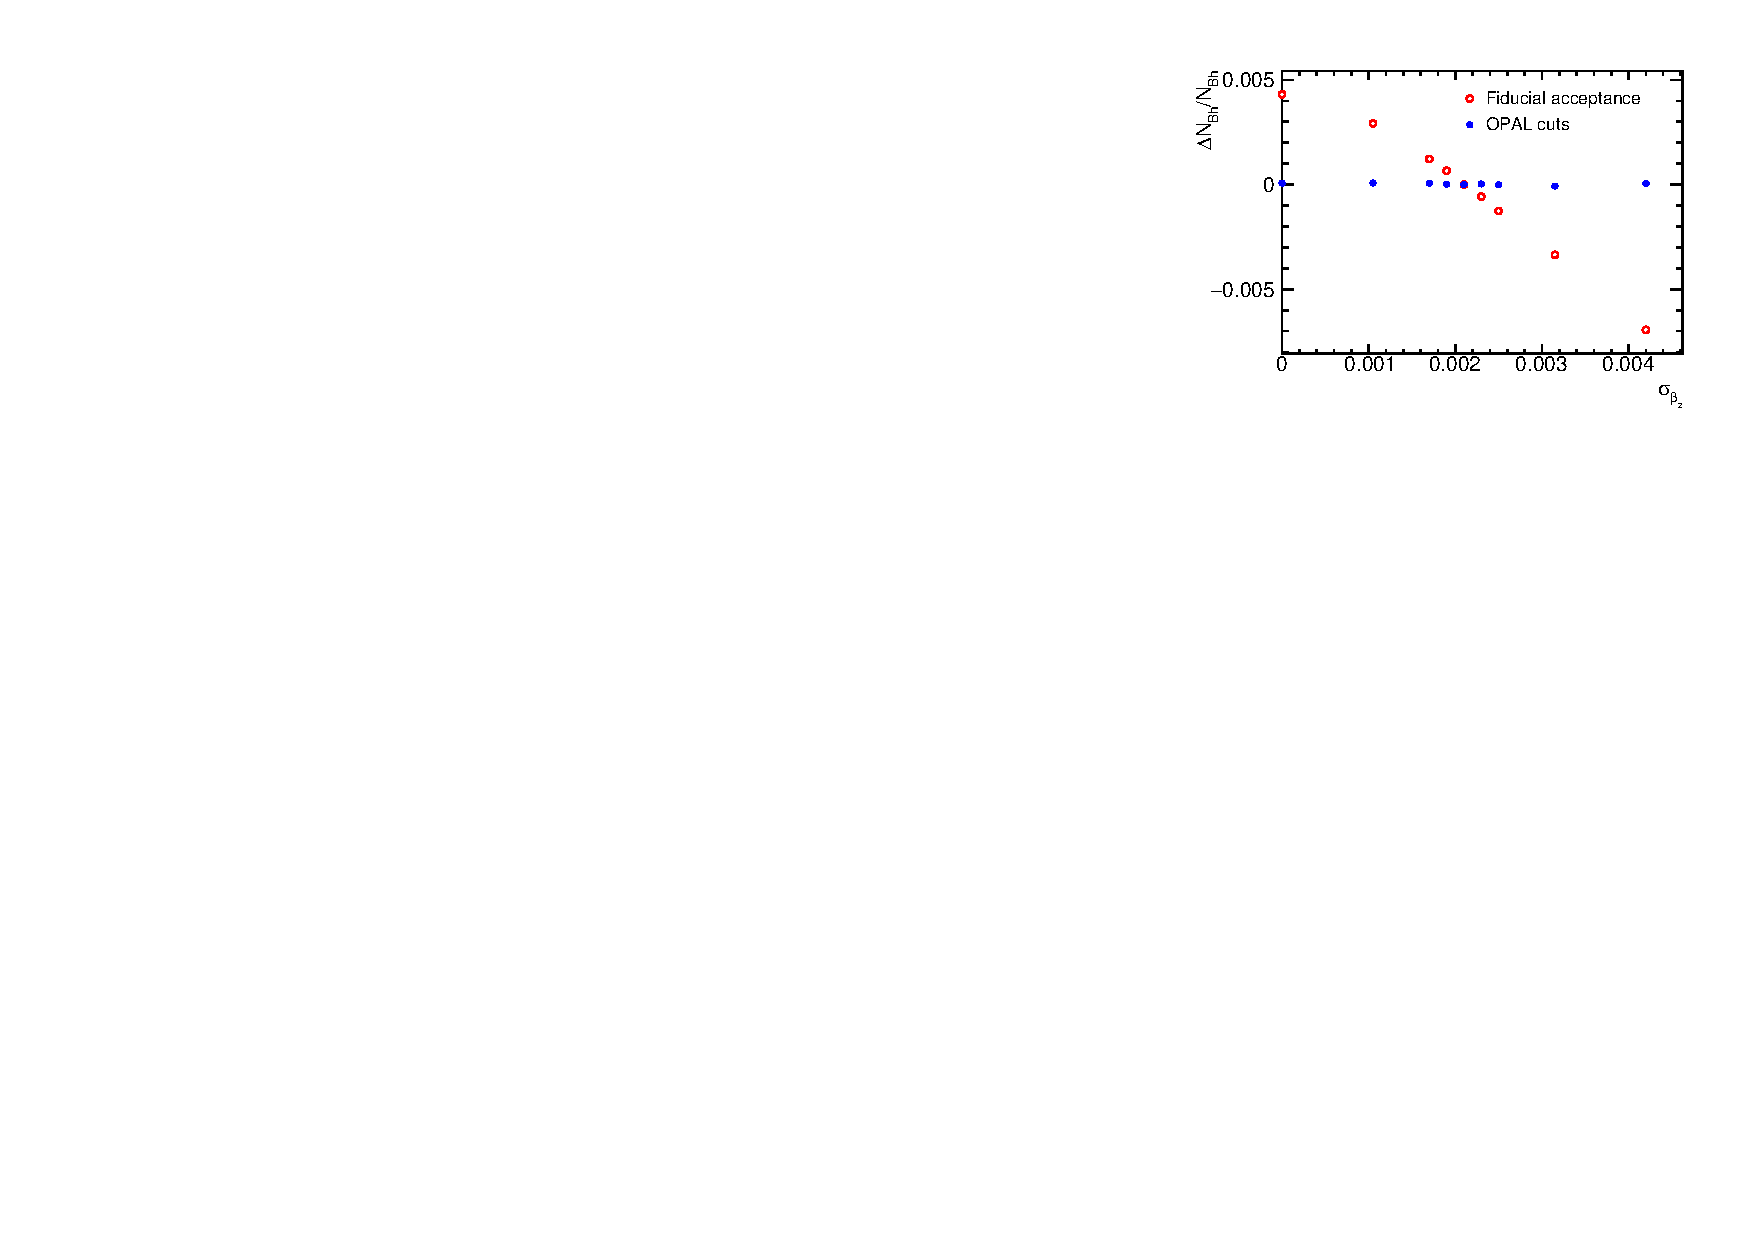
\includegraphics[width=8cm]{beamEnergySpread}
   \caption{Bhabha counting bias as a function of the width of longitudinal boost distribution due to the beam energy spread. }
   \label{fig:bes}
\end{figure}

It has been shown that most requirements on the LumiCal manufacturing and positioning, as well as on the MDI and beam delivery needed to reach the luminosity precision of 1 permille are technically feasible with the present state of the art of accelerator and detector technology. The most important challenge identified is the precision of the inner acceptance radius $r_{\text{in}}$ of LumiCal. In order to keep the luminosity precision of 1 permille, $r_{\text{in}}$ must be known to within $10\,\mathrm{\mu m}$. The precision requirement of $r_{\text{in}}$ scales linearly with the required luminosity precision, implying a correspondingly stricter requirement for the $\Zboson$-pole run.




